\begin{figure}
    \centering
    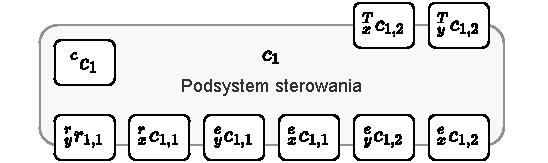
\includegraphics[width=\columnwidth]{figures/ISR-cs-model.pdf}
    \label{fig:model-cs}
    \caption{Struktura ogólna podsystemu sterowania}
\end{figure}

\begin{figure}
    \centering
    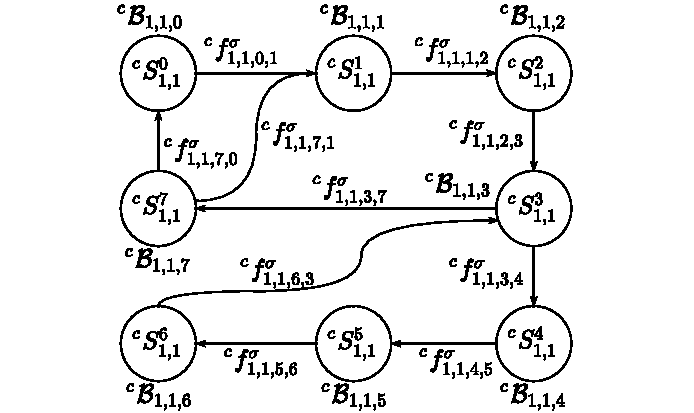
\includegraphics[width=\columnwidth]{figures/ISR-cs-behaviours.pdf}
    \label{fig:zachowania-cs}
    \caption{Automat zachowań podsystemu sterowania}
\end{figure}

Zachowania:
\begin{itemize}
    \item ${}^{c}\mathcal{B}_{1,1,0}$ - idle,
    \item ${}^{c}\mathcal{B}_{1,1,1}$ - pre-grip,
    \item ${}^{c}\mathcal{B}_{1,1,2}$ - detect-block,
    \item ${}^{c}\mathcal{B}_{1,1,3}$ - do-plan,
    \item ${}^{c}\mathcal{B}_{1,1,4}$ - grip,
    \item ${}^{c}\mathcal{B}_{1,1,5}$ - pre-store,
    \item ${}^{c}\mathcal{B}_{1,1,6}$ - detect-place,
    \item ${}^{c}\mathcal{B}_{1,1,7}$ - drop.
\end{itemize}

Stałe:\begin{itemize}
    \item $\Theta_{\mathrm{grip}}$ -- pozycja startowa do chwytu sześcianu, 
    \item $\Theta_{\mathrm{drop}}$ -- pozycja startowa do odkładania sześcianu.
\end{itemize}

Bufory komunikacyjne:
\begin{itemize}
    \item ${}^{c}c_{1,1} = [M, i, j, \Theta_{\mathrm{plan}}]$ - pamięć wewnętrzna \begin{itemize}
        \item $M$ -- macierz zer i~jedynek rozmiaru 20x20 opisująca zajętość palety,
        \item $i,j$ -- współrzędne rozważanego miejsca na palecie, numerowane od 1 do 20, 0 oznacza niewyznaczoną pozycję,
        \item $\Theta_{\mathrm{plan}}$ -- zmienna przechowująca zaplanowaną pozycję chwytu/odłożenia sześcianu.
    \end{itemize}
    
    \item ${}^{T}_{x}c_{2,1} = m \in \{ \emptyset, START \}$ - komunikat od agenta $a_{2}$,
    
    \item ${}^{r}_{y}r_{1,1} = \varphi \in \{b, p\}$ - wybór trybu pracy wirtualnego receptora kamery,
    \item ${}^{r}_{x}r_{1,1} = \Theta_{\mathrm{d}}$ - znaleziona pozycja sześcianu/miejsca w~zależności od wybranego trybu,

    \item ${}^{e}_{y}e_{1,1} = \Theta_{\mathrm{zad}}$ - zadana pozycja ramienia,
    \item ${}^{e}_{x}e_{1,1} = \Theta$ - aktualna pozycja ramienia,

    \item ${}^{e}_{y}e_{1,2} = \xi_{\mathrm{zad}} \in \{o, c\}$ - zadany stan chwytaka,
    \item ${}^{e}_{x}e_{1,2} = \xi \in \{o, c\}$ - aktualny stan chwytaka.
\end{itemize}

Wymagane funkcje pomocnicze:
\begin{itemize}
    \item $zeros()$ -- stwórz macierz 20x20 wypełnioną zerami,
    \item $isValid(\Theta)$ -- sprawdza czy $\Theta$ jest poprawną pozycją,
    \item $makePlan(\Theta, \Theta_{d})$ -- na podstawie aktualnego położenia, wykrytego położenia oraz znanej prędkości taśmociągu, określa położenie w~którym robot złapie sześcian, 
    \item $findPlace(\Theta_{d}, M)$ --na podstawie położeń wykrytych potencjalnych miejsc oraz znanej zajętości palety, określa położenie w~którym robot odłoży sześcian,
    \item $isFull(M)$ -- sprawdza czy podana macierz zajętości palety jest wypełniona.
\end{itemize}

Warunki początkowe:
\begin{itemize}
    \item ${}^{c}f^{\sigma}_{1,1,0,1} \triangleq {}^{T}_{x}c_{2,1} = START$,
    \item ${}^{c}f^{\sigma}_{1,1,1,2} \triangleq {}^{c}f^{\tau}_{1,1,1} = True$,
    \item ${}^{c}f^{\sigma}_{1,1,2,3} \triangleq isValid(\Theta_{\mathrm{d}}) = True$,
    
   
    \item ${}^{c}f^{\sigma}_{1,1,3,4} \triangleq {}^{c}f^{\tau}_{1,1,3} = True \land \Xi = o$, 
    \item ${}^{c}f^{\sigma}_{1,1,3,7} \triangleq {}^{c}f^{\tau}_{1,1,3} = True \land \Xi = c$, 

    \item ${}^{c}f^{\sigma}_{1,1,4,5} \triangleq \Xi = c$,
    \item ${}^{c}f^{\sigma}_{1,1,5,6} \triangleq {}^{c}f^{\tau}_{1,1,5} = True$,
    \item ${}^{c}f^{\sigma}_{1,1,6,3} \triangleq isValid(\Theta_{\mathrm{d}}) = True$,
    \item ${}^{c}f^{\sigma}_{1,1,7,0} \triangleq \Xi = o \land isFull(M)$,
    \item ${}^{c}f^{\sigma}_{1,1,7,1} \triangleq \Xi = o \land \neg isFull(M)$ 
\end{itemize}

Warunki końcowe:
\begin{itemize}
    \item ${}^{c}f^{\tau}_{1,1,0} \triangleq {}^{T}_{x}c_{2,1} = START $,
    \item ${}^{c}f^{\tau}_{1,1,1} \triangleq \Theta = \Theta_{\mathrm{grip}}$,
    \item ${}^{c}f^{\tau}_{1,1,2} \triangleq isValid(\Theta_{\mathrm{d}})$,
    \item ${}^{c}f^{\tau}_{1,1,3} \triangleq \Theta = \Theta_{\mathrm{plan}}$,
    \item ${}^{c}f^{\tau}_{1,1,4} \triangleq \Xi = c$,
    \item ${}^{c}f^{\tau}_{1,1,5} \triangleq \Theta = \Theta_{\mathrm{drop}}$,
    \item ${}^{c}f^{\tau}_{1,1,6} \triangleq isValid(\Theta_{\mathrm{d}})$,
    \item ${}^{c}f^{\tau}_{1,1,7} \triangleq \Xi = o$,
\end{itemize}

Funkcje przejścia w postaci matematycznej:
\begin{itemize}
    \item \textbf{idle} \begin{itemize}
        \item ${}^{c_{1,1}, c_{1,1}}f_{1,1,0} \triangleq {}^{c}c_{1,1} = [zeros(), 0, 0, \emptyset]$,
    \end{itemize} 

    \item \textbf{pre-grip} \begin{itemize}
        \item ${}^{c_{1,1}, e_{1,1}}f_{1,1,1} \triangleq {}^{e}_{y}c_{1,1} = \Theta_{\mathrm{grip}}$,
        \item ${}^{c_{1,1}, e_{1,2}}f_{1,1,1} \triangleq {}^{e}_{y}c_{1,2} = o$,
    \end{itemize}

    \item \textbf{detect-block} \begin{itemize}
        \item ${}^{c_{1,1}, r_{1,1}}f_{1,1,2} \triangleq {}^{r}_{y}c_{1,1} = b$
        \item ${}^{c_{1,1}, c_{1,1}}f_{1,1,2} \triangleq \Theta_{\mathrm{plan}}
            \begin{cases}
			    makePlan(\Theta, \Theta_{\mathrm{d}}), & isValid(\Theta_{\mathrm{d}})\\
                \emptyset, & \text{w p.p.}
		    \end{cases}$
    \end{itemize}
    
    \item \textbf{do-plan} \begin{itemize}
        \item ${}^{c_{1,1}, e_{1,1}}f_{1,1,3} \triangleq {}^{e}_{y}c_{1,1} = \Theta_{\mathrm{plan}}$
    \end{itemize}

    \item \textbf{grip} \begin{itemize}
        \item ${}^{c_{1,1}, e_{1,2}}f_{1,1,4} \triangleq {}^{e}_{y}c_{1,2} = \begin{cases}
            c, & \Theta_{\mathrm{plan}} = \Theta_{\mathrm{d}}\\
            o, & \Theta_{\mathrm{plan}} \neq \Theta_{\mathrm{d}}
        \end{cases}$
    \end{itemize}

    \item \textbf{pre-drop} \begin{itemize}
        \item ${}^{c_{1,1}, e_{1,1}}f_{1,1,5} \triangleq {}^{e}_{y}c_{1,1} = \Theta_{\mathrm{drop}}$
    \end{itemize}

    \item \textbf{detect-place} \begin{itemize}
        \item ${}^{c_{1,1}, r_{1,1}}f_{1,1,6} \triangleq {}^{r}_{y}c_{1,1} = p$
        \item ${}^{c_{1,1}, c_{1,1}}f_{1,1,6} \triangleq [\Theta_{\mathrm{plan}}, i, j] =
            \begin{cases}
			    findPlace(\Theta, \Theta_{\mathrm{d}}, M), & isValid(\Theta_{\mathrm{d}})\\
                [\emptyset, 0, 0], & \text{w p.p.}
		    \end{cases}$
    \end{itemize}

    \item \textbf{drop} \begin{itemize}
        \item ${}^{c_{1,1}, c_{1,1}}f_{1,1,7} \triangleq M[i,j] = 1$,
        \item ${}^{c_{1,1}, e_{1,2}}f_{1,1,7} \triangleq {}^{e}_{y}c_{1,2} = o$
    \end{itemize}
\end{itemize}

\begin{figure}
    \centering
    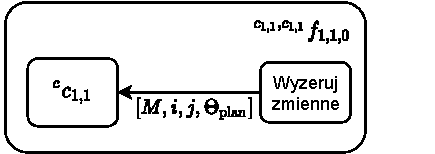
\includegraphics[width=\columnwidth]{figures/ISR-cs-fp-idle.pdf}
    \label{fig:cs-fp-idle}
    \caption{Zdekomponowana funkcja przejścia zachowania \textbf{idle} w~postaci DFD}
\end{figure}

\begin{figure}
    \centering
    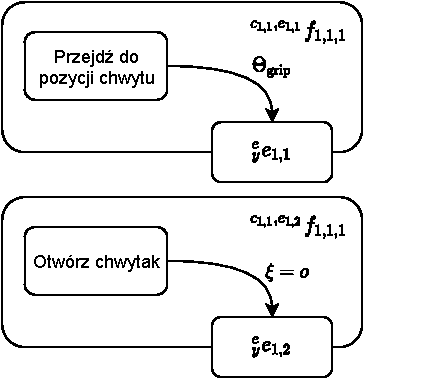
\includegraphics[width=\columnwidth]{figures/ISR-cs-fp-pre-grip.pdf}
    \label{fig:cs-fp-pre-grip}
    \caption{Zdekomponowana funkcja przejścia zachowania \textbf{pre-grip} w~postaci DFD}
\end{figure}

\begin{figure}
    \centering
    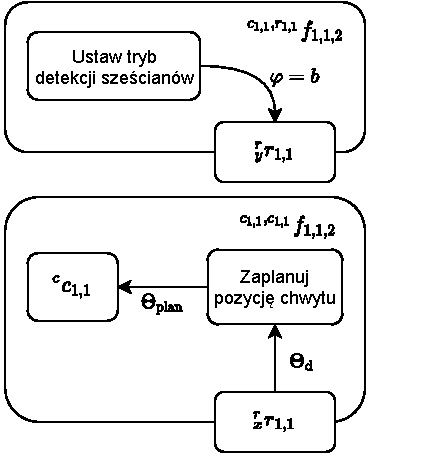
\includegraphics[width=\columnwidth]{figures/ISR-cs-fp-detect-block.pdf}
    \label{fig:cs-fp-detect-block}
    \caption{Zdekomponowana funkcja przejścia zachowania \textbf{detect-block} w~postaci DFD}
\end{figure}

\begin{figure}
    \centering
    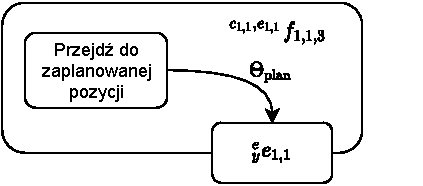
\includegraphics[width=\columnwidth]{figures/ISR-cs-fp-do-plan.pdf}
    \label{fig:cs-fp-do-plan}
    \caption{Zdekomponowana funkcja przejścia zachowania \textbf{do-plan} w~postaci DFD}
\end{figure}

\begin{figure}
    \centering
    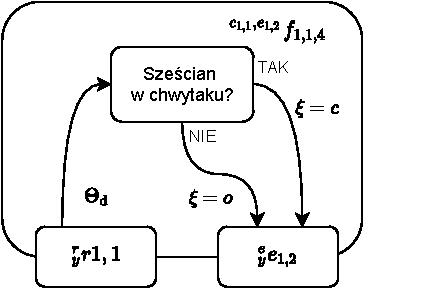
\includegraphics[width=\columnwidth]{figures/ISR-cs-fp-grip.pdf}
    \label{fig:cs-fp-grip}
    \caption{Zdekomponowana funkcja przejścia zachowania \textbf{grip} w~postaci DFD}
\end{figure}

\begin{figure}
    \centering
    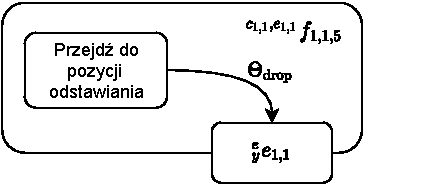
\includegraphics[width=\columnwidth]{figures/ISR-cs-fp-pre-drop.pdf}
    \label{fig:cs-fp-pre-drop}
    \caption{Zdekomponowana funkcja przejścia zachowania \textbf{pre-drop} w~postaci DFD}
\end{figure}

\begin{figure}
    \centering
    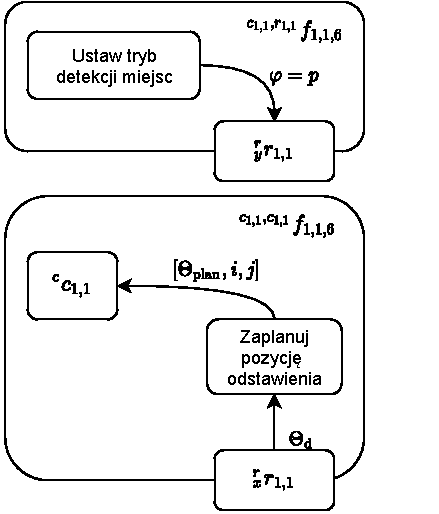
\includegraphics[width=\columnwidth]{figures/ISR-cs-fp-detect-place.pdf}
    \label{fig:cs-fp-detect-place}
    \caption{Zdekomponowana funkcja przejścia zachowania \textbf{detect-place} w~postaci DFD}
\end{figure}

\begin{figure}
    \centering
    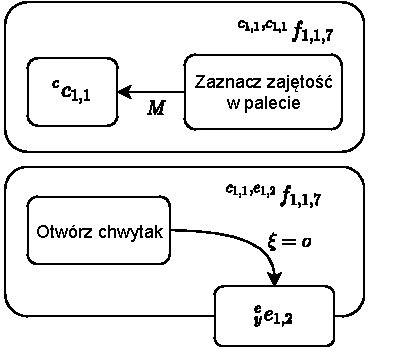
\includegraphics[width=\columnwidth]{figures/ISR-cs-fp-drop.pdf}
    \label{fig:cs-fp-drop}
    \caption{Zdekomponowana funkcja przejścia zachowania \textbf{drop} w~postaci DFD}
\end{figure}